\chapter{Identification of Architectural Erosion Issues with Static Analysis Code}
\label{cha:identification}

We can extend the solution approaches of AER issues identification in software projects based on static code analysis techniques. In this case, we implemented an analysis over a set of GitHub commits extracted from different Android projects. With the set of commits, we can identify different code fragments and implementations that could affect the architecture quality of any Android project. To get a better performance in AER issues identification, we used a set of keywords from used Word Embedding models and implemented some NLP techniques to identify the most related keywords in the commit messages. After that, we identified possible architectural smells and issues with a manual tagging process. Once the manual tagging was executed, we identified those issues and implemented a set of lint rules with the use of Android lint libraries to identify them inside any Android project. We tested that plugin and those rules with some applications to detect bad implementations in terms of architecture and quality attributes of any Android project.
The recent research about architectural erosion identification followed the same process of detection of potential issues in natural language in the commit messages from different version platforms. Furthermore, the study used different NLP techniques, like the use of static word embedding and word similarity metrics, for identifying potential words that have considerable semantic meaning in the development history of any application. With this base process, a list of potential keywords that could indicate an implemented bad architectural issue is created. However, the detection and selection process of different keywords was developed with large software Backend and Frontend projects. Those projects were implemented with traditional programming languages like Python and JavaScript. Those programming languages' documentation and support are greater than those of languages oriented toward mobile development. For this reason, it is necessary to adapt that identification methodology for the identification of potential words that have a semantic meaning inside commit messages inserted in a versioning platform for Android applications based on their source code. For this purpose, we extracted from 50 open-source Android applications and applied scraping techniques for GitHub history commit extraction. We can collect the committed messages and find similarities with the defined keywords in the research mentioned. A new version of the list of keywords will increase the accuracy of future selection and detection processes for Architectural erosion issues in the source code of Android applications.

\section{Methodology}
To solve the proposed research questions, we define a methodology to design, implement, and test a solution approach based on the static code analysis methodology mentioned in the related work. With a set of commits extracted from different open-source Android projects, we implement NLP techniques with a static Word Embedding model. After that, we define a similarity metric for finding potential keywords in the Android development context. We realized some reviews to show the accuracy with the use of the Word Embedding model. Finally, we selected a representative set of GitHub commits from the Android projects to find patterns and identify architectural smells. Once the architectural smells are found, we implement those patterns and rules into an Android Studio linter and test those with specific use cases from real Android applications and a sample Android application. We will test by comparing with other lint tools implemented for the Android Studio IDE.

\begin{figure}[h]
    	\centering
    		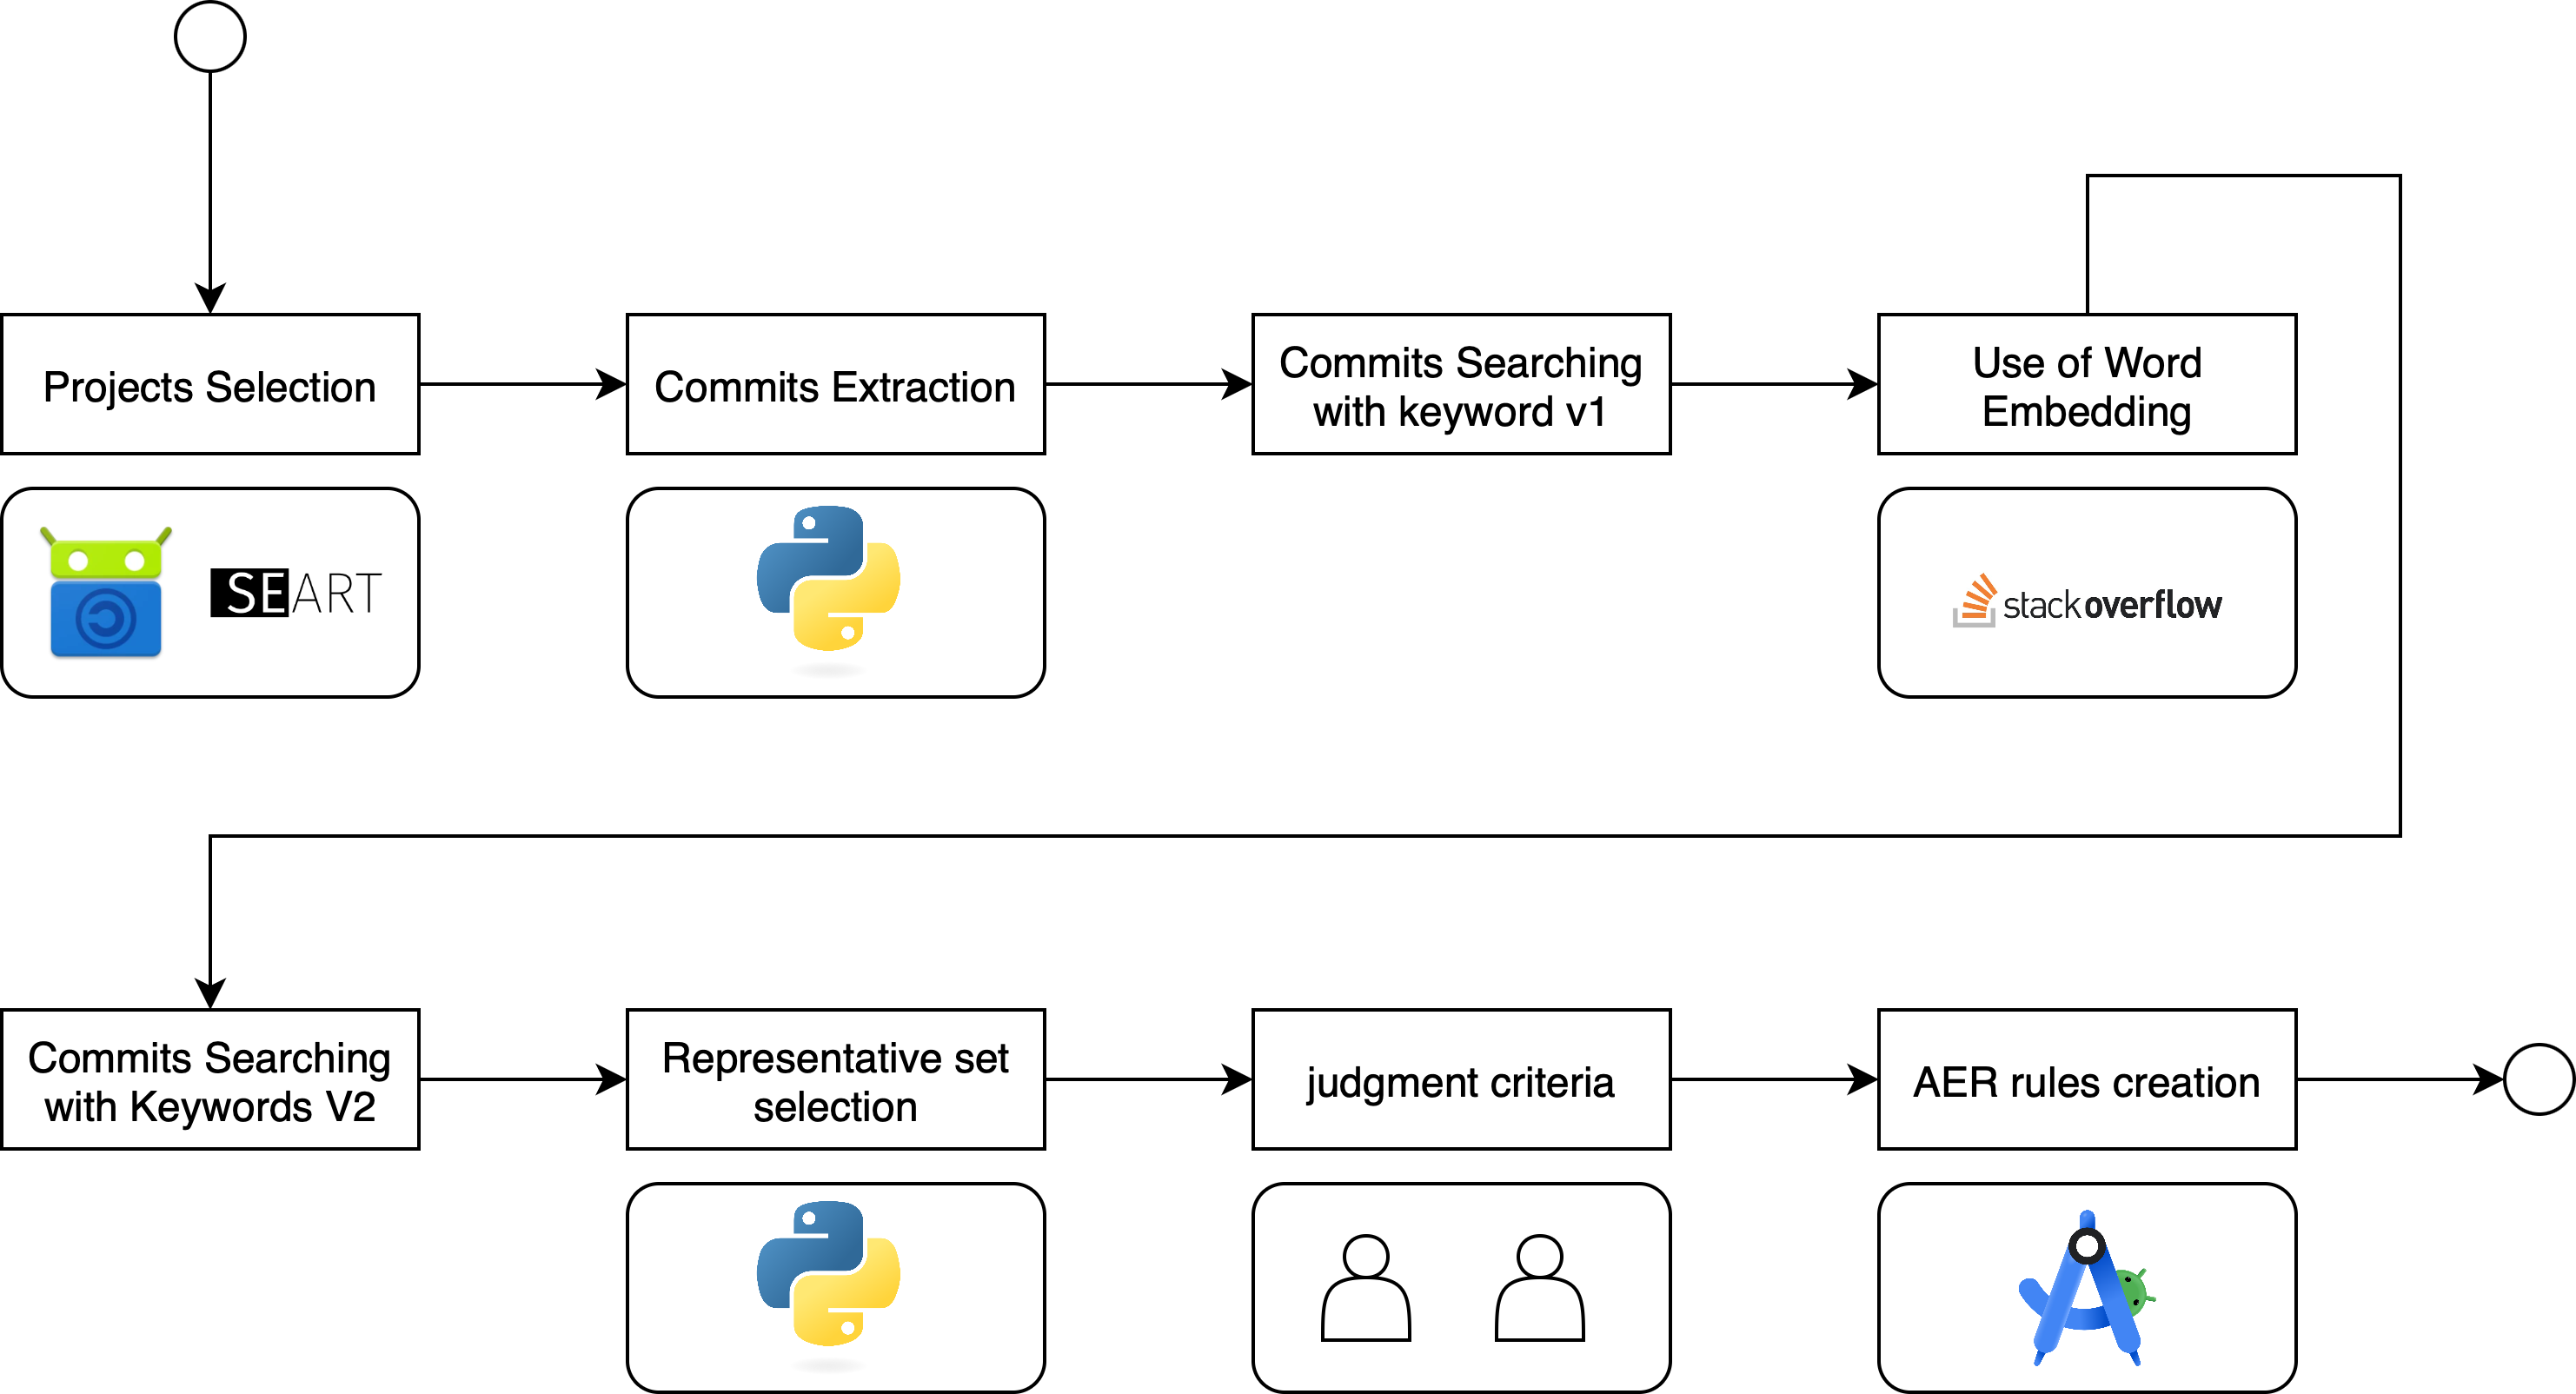
\includegraphics[scale=0.8]{/Users/juancamiloacosta/Documents/uniandes/tesis 2/thesis template repo/master-thesis-document/thesis-template/figures/workflow-1.png}
   			 \caption{Workflow for AER issues identification with Static Code Analysis techniques}
   			 \label{fig:ast}
\end{figure}


We will explain each stage of this workflow and show the results of this research compared with other proposed lint tools.

\subsection{Selection of sample Android apps}
Based on the methodology of the mentioned research, we designed a similar process of extraction and selection process for an initial version of the commits analysis. In this case, we explore different options and platforms for searching and selecting open-source Android projects whose source code is located on the GitHub versioning platform. We use two tools. The first one is SeART, a platform based on Data Mining repositories research \citet{seart_platform}. This platform has different filter features that make it possible to customize a search of different GitHub open-source projects. The customized filter for this case is to select GitHub repositories whose main programming language is Kotlin, and the number inside each repository's commit history is in the range of 1000 commits and 30000 commits. This customized filter was selected due to the opportunity to collect a large number of commits for having a strong dataset to identify potential similar keywords with a high similarity metric. With this customized filter, we select the GitHub repositories with the largest number of commits. However, the Data Mining repository techniques used are not the most effective to consider all the GitHub repository environments. For this reason, it is necessary to consider more tools for searching more GitHub repositories of open-source Android applications.



For a larger collection of Android applications for getting a better performance in AER identification and selection, we consider using an Android application searching tool. The mentioned tool is F-Droid- F-Droid is an open-source platform for searching open-source Android applications. This platform gives specific details of every Android application, and one of those details is the GitHub repository URL. With that attribute and the type of license declared in the F-Droid platform.

Once the applications are selected, we implemented a program based on web scraping techniques with the PyDriller library and built a dataset with the main features of each commit in the GitHub repository of the source code of each Android application.

\begin{figure}[h]
    	\centering
    		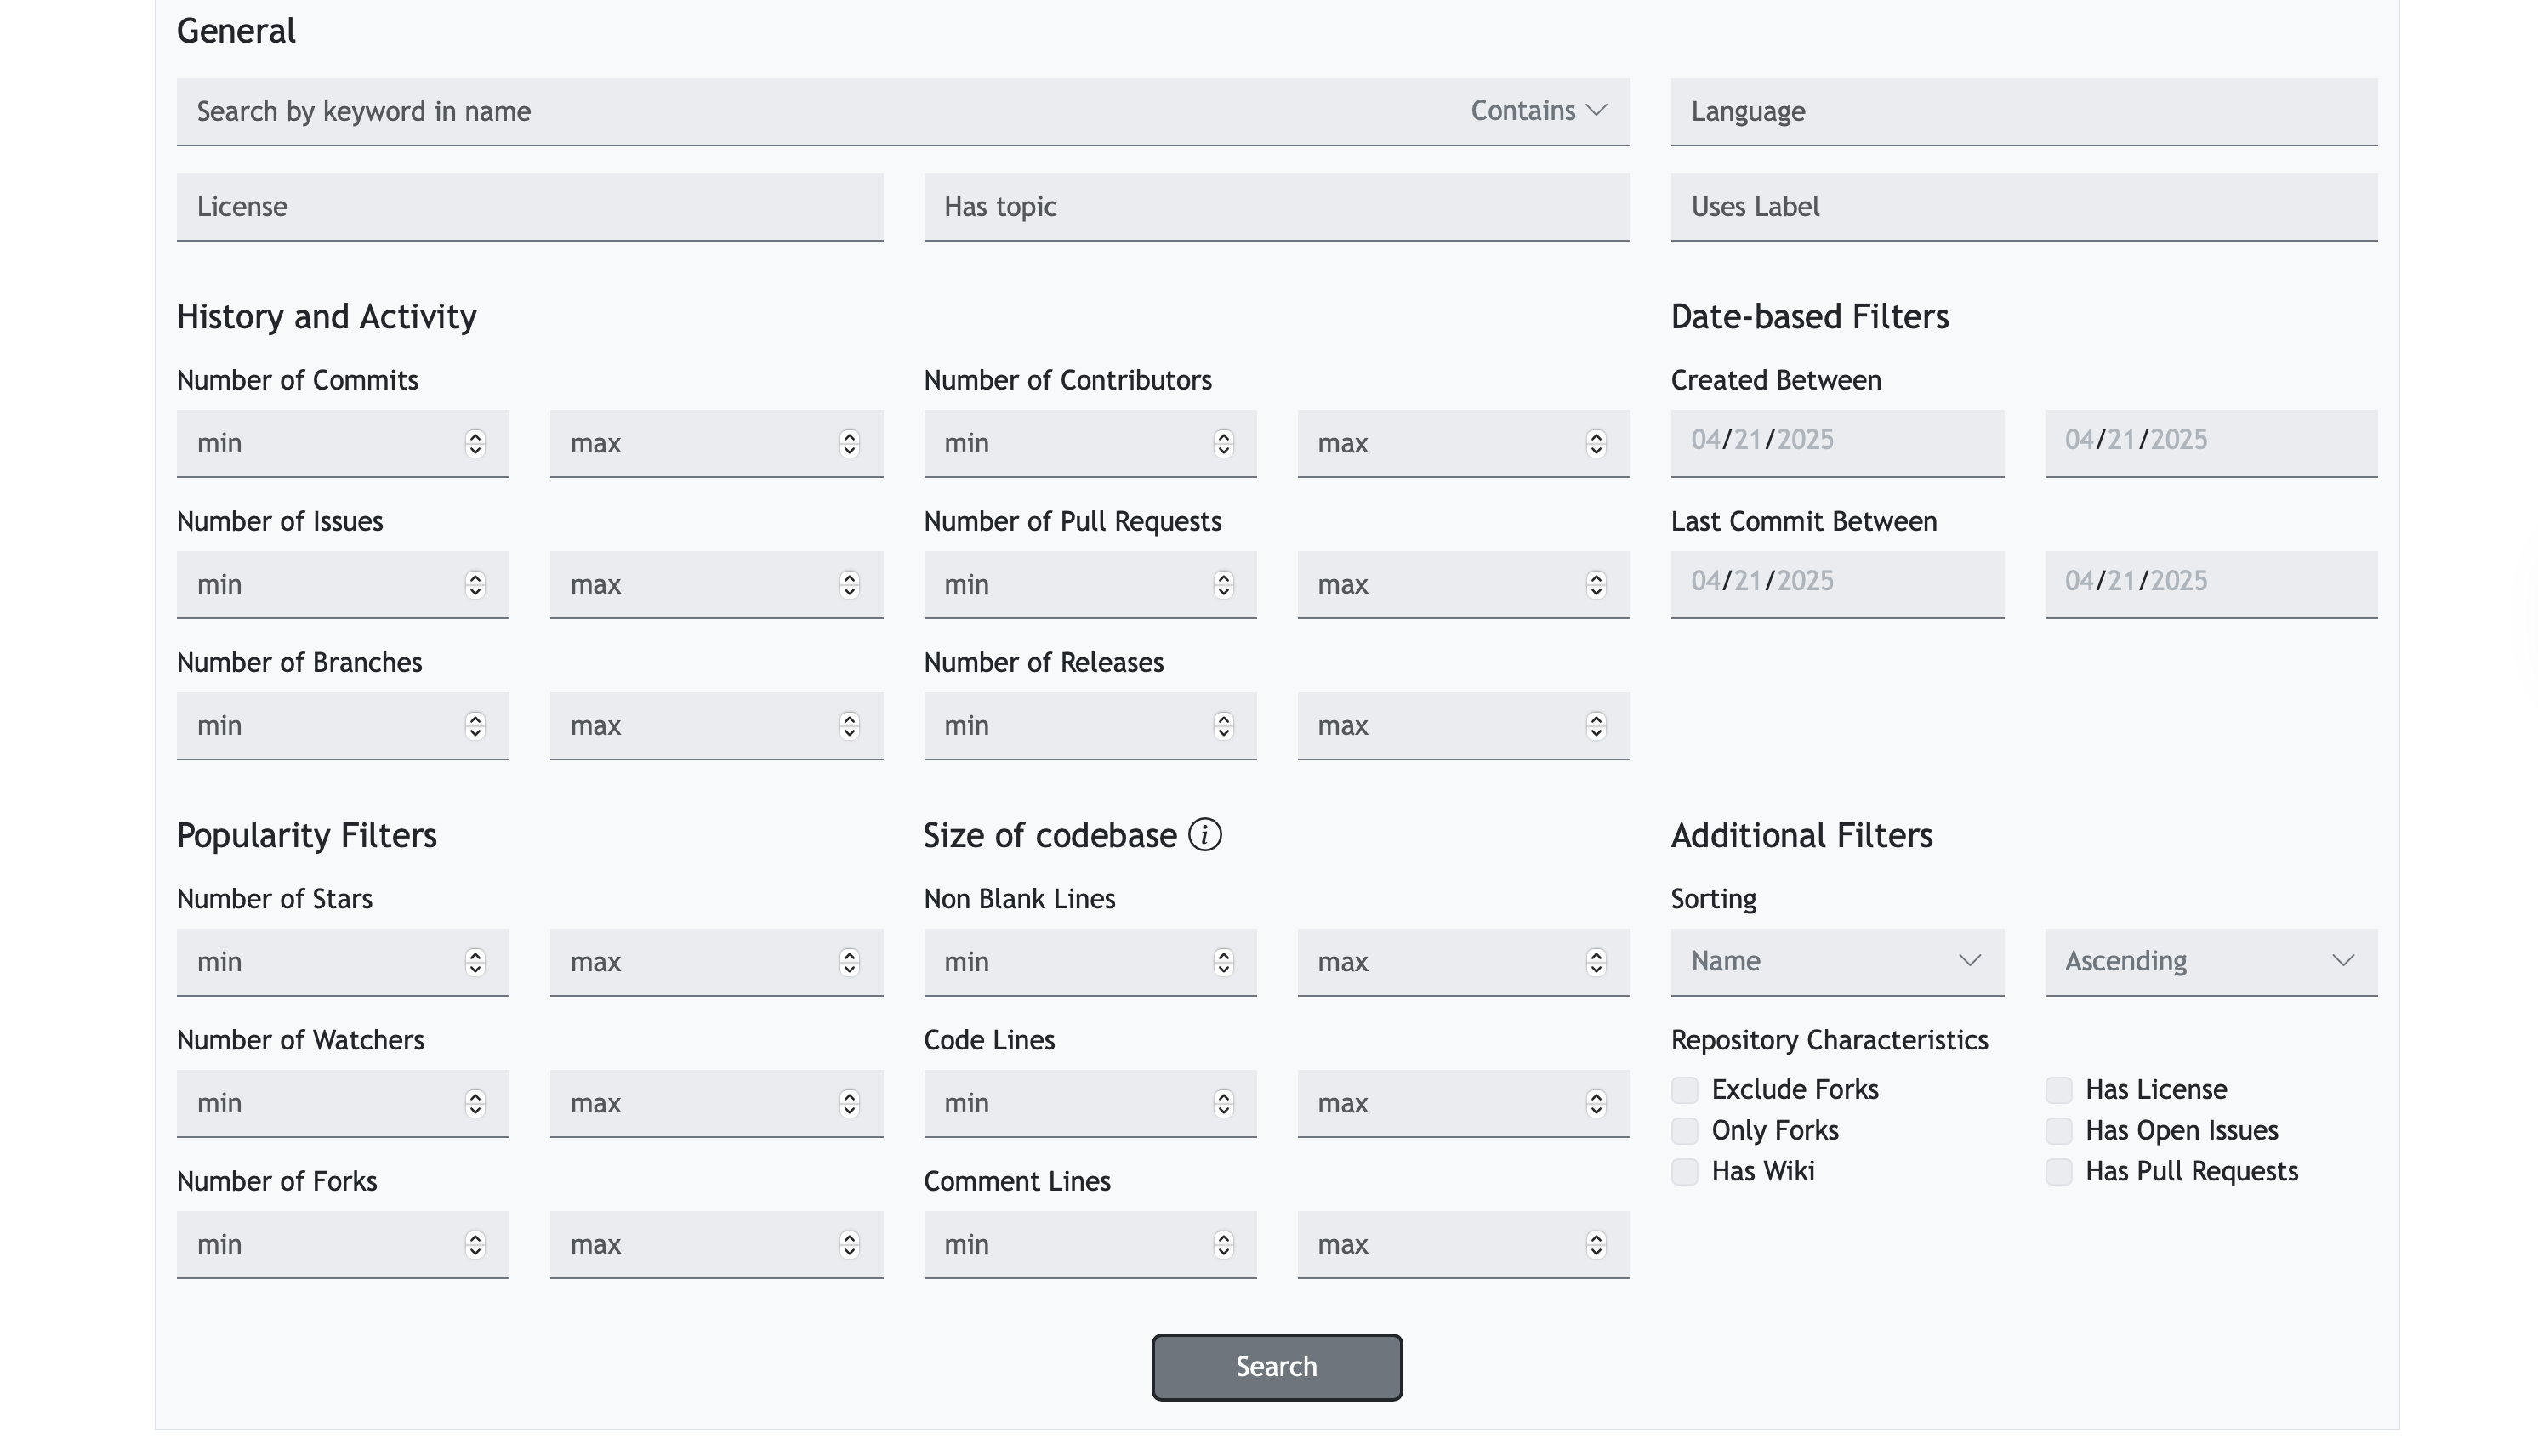
\includegraphics[scale=0.3]{/Users/juancamiloacosta/Documents/uniandes/tesis 2/thesis template repo/master-thesis-document/thesis-template/figures/seART.png}
   			 \caption{seART platform for GitHub repositories searching \citet{seart_platform} }
   			 \label{fig:ast}
\end{figure}

\subsection{Word Embedding and Similarity Criteria}
With the collected set of commits from the mentioned Android apps collection, we made a preprocessing process for the developers' messages of those commits. In this case, we implemented a preprocessing flow with stemming, lemmatizing, and stop word removal. After that, we used the static pre-trained Word Embedding model, trained on 2 million Stack Overflow posts. With that model, we extracted the numerical representation of each word in the vocabulary of the GitHub commits dataset of selected Android applications. With the cosine similarity metric, we extracted the most similar words based on the keywords found in the related work.


\subsection{Architectural erosion symptoms Identification}
Based on the last research, architectural erosion insight identification consists of a deep analysis of information based on development judgments. This judgment can be extracted from different software versioning systems, like OpenStack, a software versioning platform for large-scale software projects, or GitHub, the most used software versioning platform. From those messages, we can classify and tag different code changes through code differences between code changes over time. In this process, the use of different Natural Language Processing (NLP) techniques, to find a standard architectural erosion commit definition. One innovative idea is to employ pre-trained Word Embeddings in software development contexts for potential words that could indicate an implemented architectural violation in server-side applications. The use of embeddings and word similarity metrics like Cosine Similarity allows us to calculate the similarity between the word embedding's numerical representation for every word, since semantic function. With this study, we can standardize the main cases of architectural erosion, the different metrics that could be identified in a software project, and potential solution approaches.
With those NLP metrics, we can use them to create discriminatory models for issue detection. However, in an Android context, the architectural erosion identification hasn't been enough to standardize a set of rules for detecting it in software source code due to the Backend and Frontend solution approaches implemented in the study software projects (the two main projects are developed in Python).
With the results of the papers extracted in the first related research overview, we can find a set of keywords extracted for the developer's code messages that indicates a potential architectural erosion issue in the implementation, that study was realized with the developer's judges and messages extracted from different version platforms like OpenStack (previously mentioned) and Github, the most popular and used versioning platform. In this case, the project had as a reference four large open-source software projects; all applications are server-side applications. Around 50 keywords were mentioned as potential keywords that indicate an air issue.
However, the words were extracted for Backend development purposes. For this reason, we use the same word extraction approach in a mobile context. During this process, we extracted from 50 open-source Android applications published around 470k GitHub commits. This is enough detail to make a preprocessing of vocabulary implemented in each GitHub commit and create new rules that could be implemented with custom lint check rules. That topic will be treated in the next chapter.

\subsubsection{Extracting keywords from Android Context}
To get a large set of commits to analyze, we found some platforms with open-source Android projects to extract their code and analyze their commits. We used different platforms based on the
Based on the last-mentioned research, it is possible to find potential keywords that indicate an issue or an insight inside a code implementation, with the help of NLP techniques, through similarity measurements like cosine similarity (mentioned in the definitions chapter) and pre-trained Word Embeddings, due to the numerical representation of each word of the generated vocabulary in a specific context. First, we use the PyDriller library \citet{pydriller}, a useful library for repository mining, for getting the code source and its attributes of different open-source Android projects made in Kotlin. The selected projects were extracted from different open-source Android project catalogs like F-Droid and other data mining repositories found with different filters like development programming language used, number of commits, and keywords in the selection criteria \citet{fdroid,repository_mining}. In the first overview, we extracted 50 Android projects that have around 470K commits. With these commits, we made a text pre-processing to build a standard vocabulary and tokenize with the help of the NLTK library \citet{nltk}, a library for making NLP operations like tokenization, lemmatization, and stemming.

\begin{table}[H]
    \centering
    \begin{tabular}{|c|}
        \hline
        Keyword \\
        \hline
         architecture, architectural, structure, structural, \\
         layer, design, violate, violation, deviate, deviation,\\
         inconsistency, inconsistent, consistent, mismatch, diverge,\\
         divergence, divergent, deviate, deviation, architecture,\\
         layering, layered, designed, violates, violating, violated,\\
         diverges, designing, diverged, diverging, deviates, deviated, \\
         deviating, inconsistencies, non-consistent, discrepancy, deviations, \\
         modular, module, modularity, encapsulation, encapsulate, \\
         encapsulating, encapsulated, intend, intends, intended, \\
         intent, intents, implemented, implement, implementation,\\
         as-planned, as-implemented, blueprint, blueprints, mismatch,\\
         mismatched, mismatches, mismatching\\
         \hline
    \end{tabular}
    \caption{List of initial Keywords extracted of the mentioned related work}
    \label{tab:my_label}
\end{table}

\begin{table}[H]
    \centering
    \begin{tabular}{|c|c|}
        \hline
        Column & Description \\
        \hline
        Name Repo & Name of the GitHub repository of Android project source code \\
        \hline
        Url Repo & GitHub URL from source code repository \\
        \hline
       Commit Message & Message of a specific commit in GitHub commits history of each Android project \\
       \hline
       Commit Hash & Hash from GitHub commit, essential for the commits analysis process \\
       \hline
       File Name & List of GitHub commit modified file names \\
       \hline
       Code Changes & String with the modified source code of each GitHub commit \\
       \hline
    \end{tabular}
    \caption{Features of commits dataset and their description}
    \label{tab:my_label}
\end{table}

With all the corpus data from GitHub commits, we implement a text cleaning process, removing stop words and performing stemming. Due to the lemmatization process being less effective in a technical context, some words do not have their respective lexical roots, so the tokenizer would not consider those words. The stemming process is useful for semantic word derivation control. This process is essential because a lot of words do not have semantic relevance in each GitHub commit, so consider that words could affect similarity metrics. With the processed words, we use a pre-trained Word Embedding based on millions of Stack Overflow posts. With the Gensim library \citet{gensim}, we can load the Word Embedding model, get a numerical representation of each selected word, and use the cosine similarity metric to find similar words from the previous keywords. When the metric is generated, we select the 10 most similar words based on that metric.
In the first overview implementation, we found around 5000 relevant commits with the updated keywords list. For efficient selection criteria, we extract a representative subset based on a weighted average made by the word frequency in the corpus text. With the first selection of a representative set, we extracted 357 GitHub commits. 


\begin{table}[H]
    \centering
    \begin{tabular}{|c|c|}
    \hline
       Word  & Cosine Similitude Average Value \\
       \hline
        \texttt{notion} & 0.2674 \\
        \hline
        \texttt{respect} & 0.2627 \\
        \hline
        \texttt{formal} & 0.2482 \\
        \hline
        \texttt{high-level} & 0.2437 \\
        \hline
        \texttt{tend} & 0.2342 \\
        \hline
        \texttt{rigid} & 0.2315 \\
        \hline
        \texttt{kind} & 0.2256 \\
        \hline
        \texttt{stronger} & 0.2243 \\
        \hline
        \texttt{non-linear} & 0.2227 \\
        \hline
        \texttt{sane} & 0.2198 \\
        \hline
    \end{tabular}
    \caption{Top 10 newfound words since Word Embedding cosine similarity metric}
    \label{tab:my_label}
\end{table}

With this approach, it is possible to find potential words written in a development context that could indicate a potential issue related to different kinds of functional and non-functional requirements that a software project includes in its architectural design and its standards. This detection approach has many different development areas to detect different problems found in a software project. The future work related to this approach will be discussed in the next chapters.
\endinput